\subsection{The heat equation}

We want to use a finite-difference (Euler) method to find an approximate solution of the heat equation
\begin{equation}
  T_t = k T_{xx}
  \label{eq_heat_equation}
\end{equation}
with the initial condition
\begin{equation}
  T(x,0) = 100 \sin(\pi x / L),
  \label{eq_initial_condition}
\end{equation}
and boundary conditions
\begin{equation}
  T(0,t) = T(L,t) = 0
  \label{eq_boundary_conditions}
\end{equation}
for $L = 1 \ m$. Here we use a short notation for the derivatives: $T_t = \frac{\partial T}{\partial t}$.


\subsection{The recurrence relation}

Our goal is to find a recurrence relation that will allow us to calculate the value of temperature iteratively at each time step. In order to find this recurrence relation we use approximations for the derivatives. The time derivative approximation is
\[
  T_t(x, t) \approx \frac{T(x, t + \Delta t) - T(x, t)}{\Delta t},
\]
with the corresponding approximate expression
\begin{equation}
  (T_t)_j^n = \frac{T_j^{n + 1} - T_j^{n}}{\Delta t},
  \label{eq_time_derivative_approximation}
\end{equation}
where the $j$ is the position index and $n$ is the time index:
\begin{align*}
  j &= 1, 2, \dots, n_x \\
  n &= 1, 2, \dots, n_t,
\end{align*}
with $n_x$ and $n_t$ being the total number of position and time values respectively.
Similarly, the approximate expression for the second position derivative is:
\begin{equation}
  (T_{xx})_j^n = \frac{T_{j+1}^n - 2 T_{j}^n + 2T_{j-1}^n}{\Delta x^2}.
  \label{eq_space_derivative_approximation}
\end{equation}
Next, we substitute Equations \ref{eq_time_derivative_approximation} and \ref{eq_space_derivative_approximation} into \autoref{eq_heat_equation}:
\[
  \frac{T_j^{n + 1} - T_j^{n}}{\Delta t} = k \frac{T_{j+1}^n - 2 T_{j}^n + 2T_{j-1}^n}{\Delta x^2}.
\]
Finally, we solve for $T_j^{n + 1}$ and find the recurrence relation that we wanted
\begin{equation}
  \boxed{ T_j^{n + 1} = T_j^{n} + \alpha \big( T_{j+1}^n - 2 T_{j}^n + 2T_{j-1}^n \big), \quad \alpha = k \frac{\Delta t}{\Delta x^2}. }
  \label{eq_recurrence_relation_heat_eq}
\end{equation}


\subsection{Writing the code}

Next, we write Fortran code to solve the heat equation (\autoref{eq_heat_equation}). The code is shown in shown in \autoref{code_solve_heat_equation}.


\noindent\begin{minipage}{\linewidth}
\begin{lstlisting}[caption={Solving a heat equation with forward-difference method (\code{heat\_equation.f90}).},frame=tlrb,label={code_solve_heat_equation}, numbers=left, firstnumber=77]
! Assign evenly spaced x values
call linspace(x0, x1, x_points)

! Set initial conditions
data(:, 1) = 100._dp * sin(pi * x_points / l)

! Set boundary conditions
data(1, :) = 0
data(nx, :) = 0

! Calculate numerical solution using forward differencing method
do n = 1, nt - 1
    data(2:nx-1, n + 1) = data(2:nx-1, n) + &
        alpha * (data(3:nx, n) - 2 * data(2:nx-1, n) + data(1:nx-2, n))
end do
\end{lstlisting}
\end{minipage}

On \code{Line 77} we assign evenly spaced values between $0$ and $1$ for the x-coordinate and store then in the \code{x\_points} array. The number of the values \code{nx} are supplied to the program by the user.

Next, on \code{Line 81} use the initial condition from \autoref{eq_initial_condition}. Our temperature values are stored in a 2D array variable called \code{data}. Here we assign the temperatures to all the x-values corresponding to the first time index $n=1$.

Similarly, on \code{Line 77} and \code{78} we use the boundary conditions (\autoref{eq_boundary_conditions}) by assigning zero temperatures to the ends of the rod. This is done by assigning zero for all time indexes in the \code{data} array corresponding to first (1) and last (\code{nx}) x-index.

Finally, on \code{Lines 88-91} we iterate over time indexes (\code{n}) and use the recurrence relation from \autoref{eq_recurrence_relation_heat_eq} to assign the temperature value for the next time index (\code{n + 1}) using the temperatures that were calculated for the previous step for the time index (\code{n}).

On \code{Lines 89-90} are using a so-called ``vectorized'' indexing syntax for the x-coordinate, such as \code{2:nx-1}. This allows the program to use SIMD processor instructions that perform multiple operations in one cycle. These instructions take advantage of the fact that x-values are located contiguously in memory (Fortran arrays are column-major, meaning the values from the first index of an array are stored one after another in memory). This index notation will make out calculation multiple times faster (this speed increase depends on type of SIMD instructions implemented in a specific processor) compared to an alternative implementation where we would iterate over the $x$ values using a loop.


\subsection{Running the program and making plots}

Instructions for compiling, running the program and plotting its results are located in the README.md file that comes with the source code.



\subsection{Approximate solution and errors}

We look at the approximate solution produced by our program by first plotting the solution for small number of x values ($nx = 5$) on \autoref{fix_solution_nx_5_alpha_0_1}.
\begin{figure}[H]
  \centering
  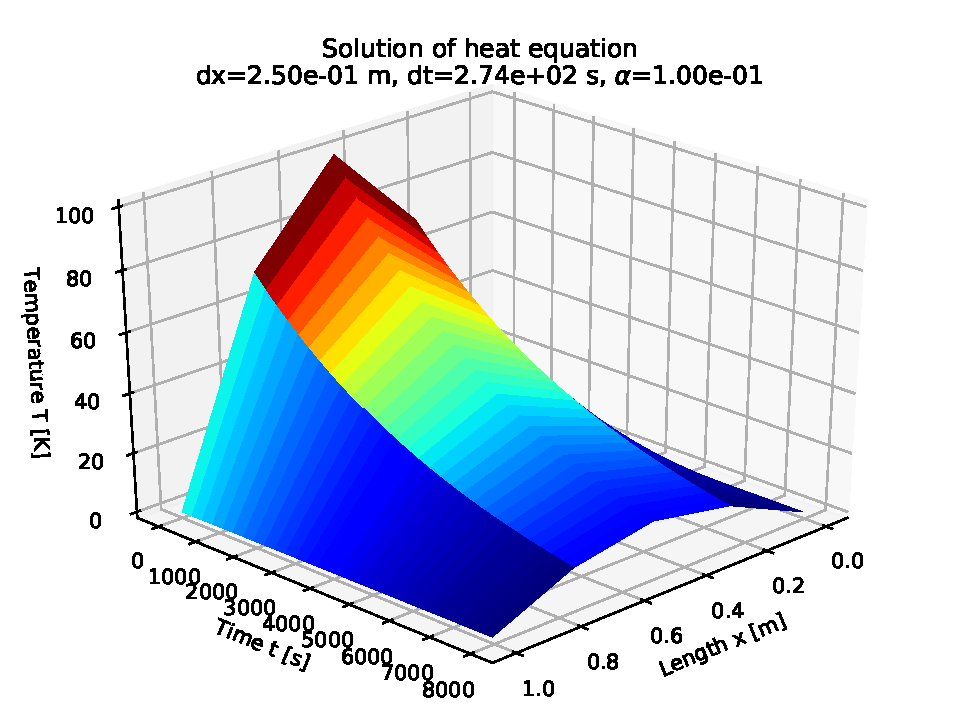
\includegraphics[width=1.0\textwidth]{figures/solution_1_00e_01.pdf}
  \caption{Approximate solution to the heat equation for $nx=5$ and $\alpha = 0.1$.}
  \label{fix_solution_nx_5_alpha_0_1}
\end{figure}
We can see from \autoref{fix_solution_nx_5_alpha_0_1} that the the temperature of the rod decreases from a sinusoidal distribution with time, and the ends remain at $T=0$, as expected. 

The corresponding errors are shown on \autoref{fix_errors_nx_5_alpha_0_1}. The errors were found by calculating the absolute value of the difference between the approximate solution and the exact solution, which is given by equation
\[
  T(x,t) = 100 e^{- \pi^2 k t / L^2} \sin(\pi x / L).
\]
We can see from \autoref{fix_errors_nx_5_alpha_0_1} that the errors are increasing with time, and that the errors are larger near the center of the rod. We can see that the errors reach peak values of about $10 K$ at $t \approx 3000 \ s$.
\begin{figure}[H]
  \centering
  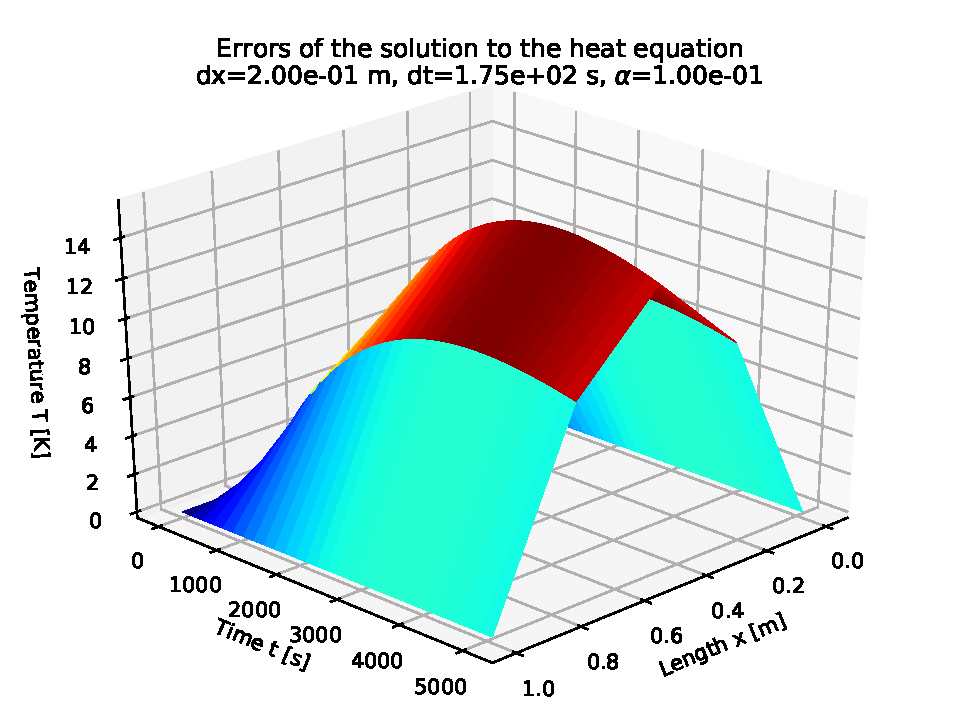
\includegraphics[width=1.0\textwidth]{figures/errors_alpha_1_00e_01.pdf}
  \caption{The absolute errors of the approximate solution of the heat equation for $nx=5$ and $\alpha = 0.1$.}
  \label{fix_errors_nx_5_alpha_0_1}
\end{figure}


\subsubsection*{Solution for $20$ position steps}

Next, we use larger amount of position steps, $nx = 20$ and $\alpha = 0.25$. The solution is shown on \autoref{fix_solution_nx_20_alpha_0_2_5}. We have calculated the solution for $300$ time steps ($nt = 300$).
\begin{figure}[H]
  \centering
  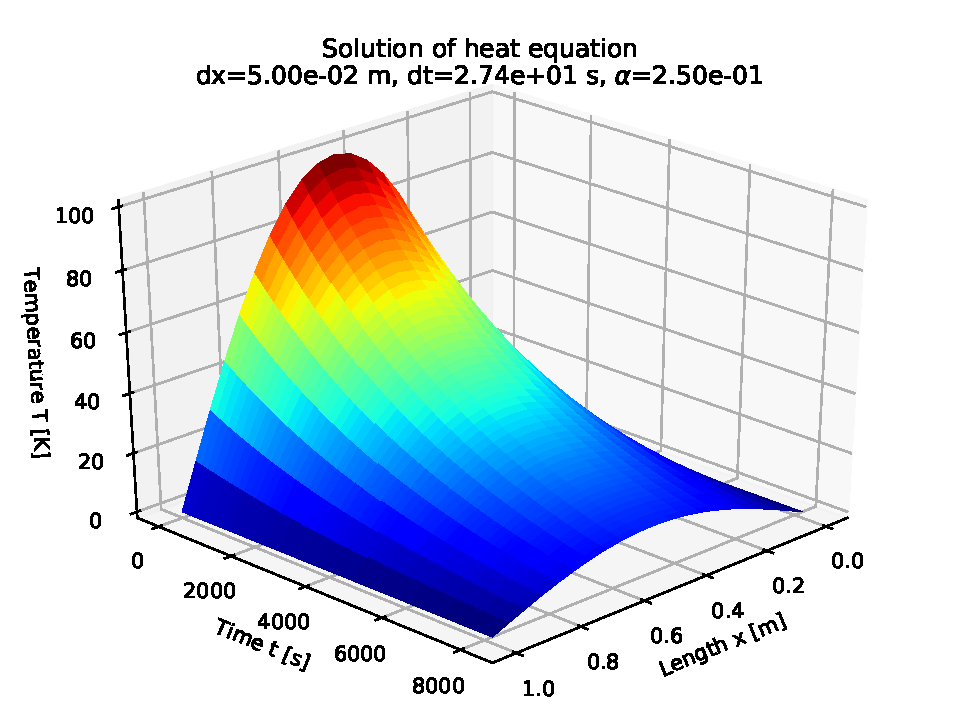
\includegraphics[width=1.0\textwidth]{figures/solution_2_50e_01.pdf}
  \caption{Approximate solution to the heat equation for $nx=20$ and $\alpha = 0.25$.}
  \label{fix_solution_nx_20_alpha_0_2_5}
\end{figure}
The general shape of the solution is not unlike the one we found for $nx=5$. We can see that the new $nx=20$ solution is smoother, which can be explained by smaller steps for position and time. The errors of the approximate solution for $nx=20$ are shown on \autoref{fix_errors_nx_20_alpha_0_2_5}.
\begin{figure}[H]
  \centering
  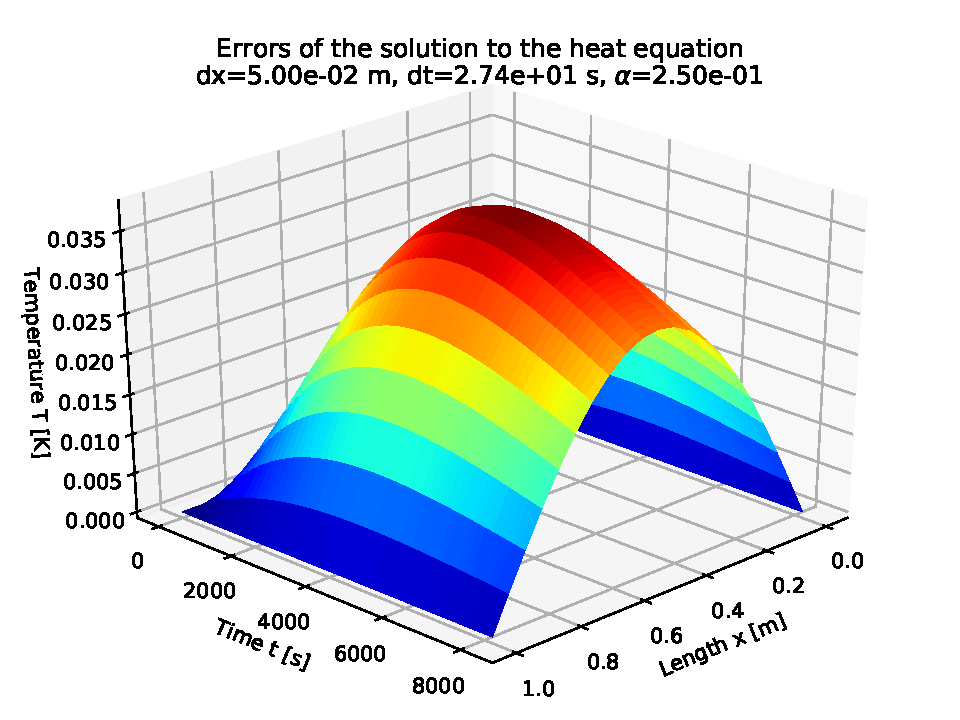
\includegraphics[width=1.0\textwidth]{figures/errors_alpha_2_50e_01.pdf}
  \caption{The errors of the approximate solution to the heat equation for $nx=20$ and $\alpha = 0.25$.}
  \label{fix_errors_nx_20_alpha_0_2_5}
\end{figure}
We can see similar distribution of errors as before. This time, however, the peak values of errors are about $3$ times smaller, reaching maximum values of about $3.5 \ K$.


\subsection{Solution for $\alpha=0.65$}

Here we want to see how values of $\alpha$ parameter affect the solution. Specifically, we use $\alpha = 0.65$ while keeping the same number of position steps ($nx=20$). The solution is shown on \autoref{fix_solution_nx_20_alpha_0_6_5}.
\begin{figure}[H]
  \centering
  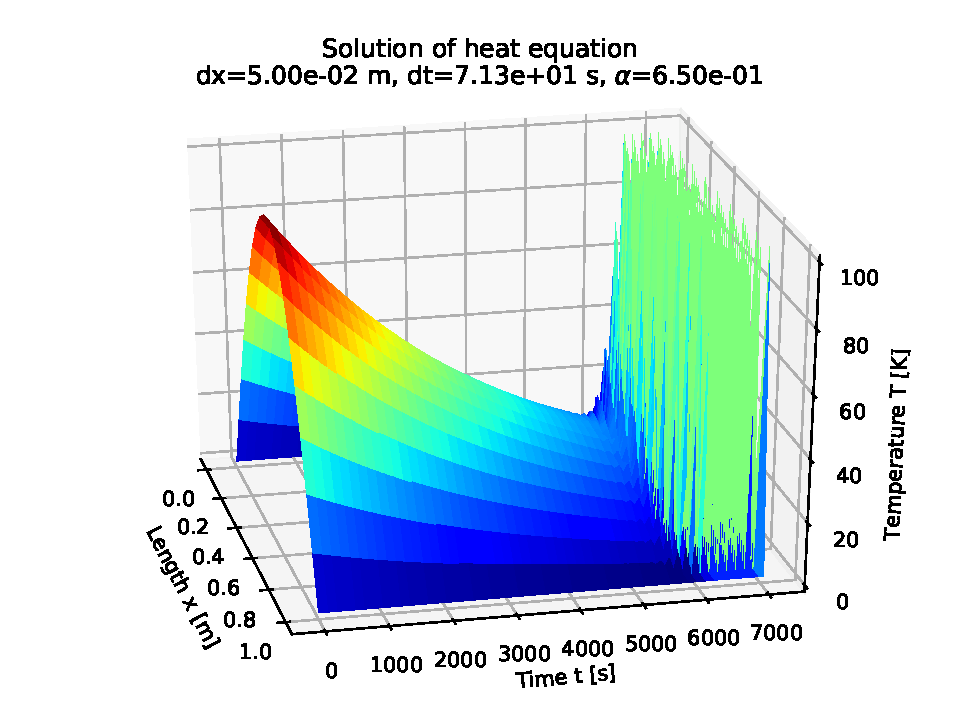
\includegraphics[width=1.0\textwidth]{figures/solution_6_50e_01.pdf}
  \caption{Approximate solution to the heat equation for $nx=20$ and $\alpha = 0.6.5$, showing signs of numerical instability from $t \approx 5500 \ s$.}
  \label{fix_solution_nx_20_alpha_0_6_5}
\end{figure}
We can see form \autoref{fix_solution_nx_20_alpha_0_6_5} that initially, the program produces results similar to the previous case with $\alpha=0.25$. However, after about $t \approx 5500 \ s$, the $\alpha=0.65$ solution shows large fluctuations in temperature. These result are unrealistic, since the rood cools down with time, and it can not heat up in random locations without an external supply of energy.

These problems in our numerical solution are likely to come from unbounded growth of rounding errors. A more detailed stability analysis using Von Neumann method is needed to show that the forward-difference method of solving \autoref{eq_heat_equation} is unstable for $\alpha > 0.5$. This condition limits our choice of the position steps: we can not make $\Delta x$ as small as we like for same values of $\Delta t$. Fortunately, there are alternative methods of solving \autoref{eq_heat_equation}, such as backward-difference and Crank-Nicolson methods, that are always stable for any choice of $\Delta x$ and $\Delta t$.



\subsection{Conclusion}

We used forward-difference (Euler) method and solved a heat equation with initial and boundary conditions. We have found that smaller position and time steps result in smaller errors. However, we have also found that making our position step too small results in unlimited growth of errors.